\recipe{Banana Milkshake}
\label{recipe:banana_milkshake}
\worktime{15 minutes}
\totaltime{15 minutes}
\makes{Makes enough for three large glasses}
\source{From Jack} % Jack Beda (Bea's 1st year med housemate)

\begin{ingredients}
  \item 6 bananas, frozen
  \item Yoghurt, \SI{300}{\gram}
  \item Milk, about \SI{300}{\gram}
  \item Garnish: cinnamon, \SI{1}{\teaspoon}
\end{ingredients}

\begin{method}
  Blend together all ingredients, adding more milk as needed to achieve desired consistency.

  Garnish with cinnamon and serve.
\end{method}


\begin{figure}[h]
  	\centering
  	
  	\begin{tikzpicture}
  		% Save the image in a box to get its dimensions
  		\sbox0{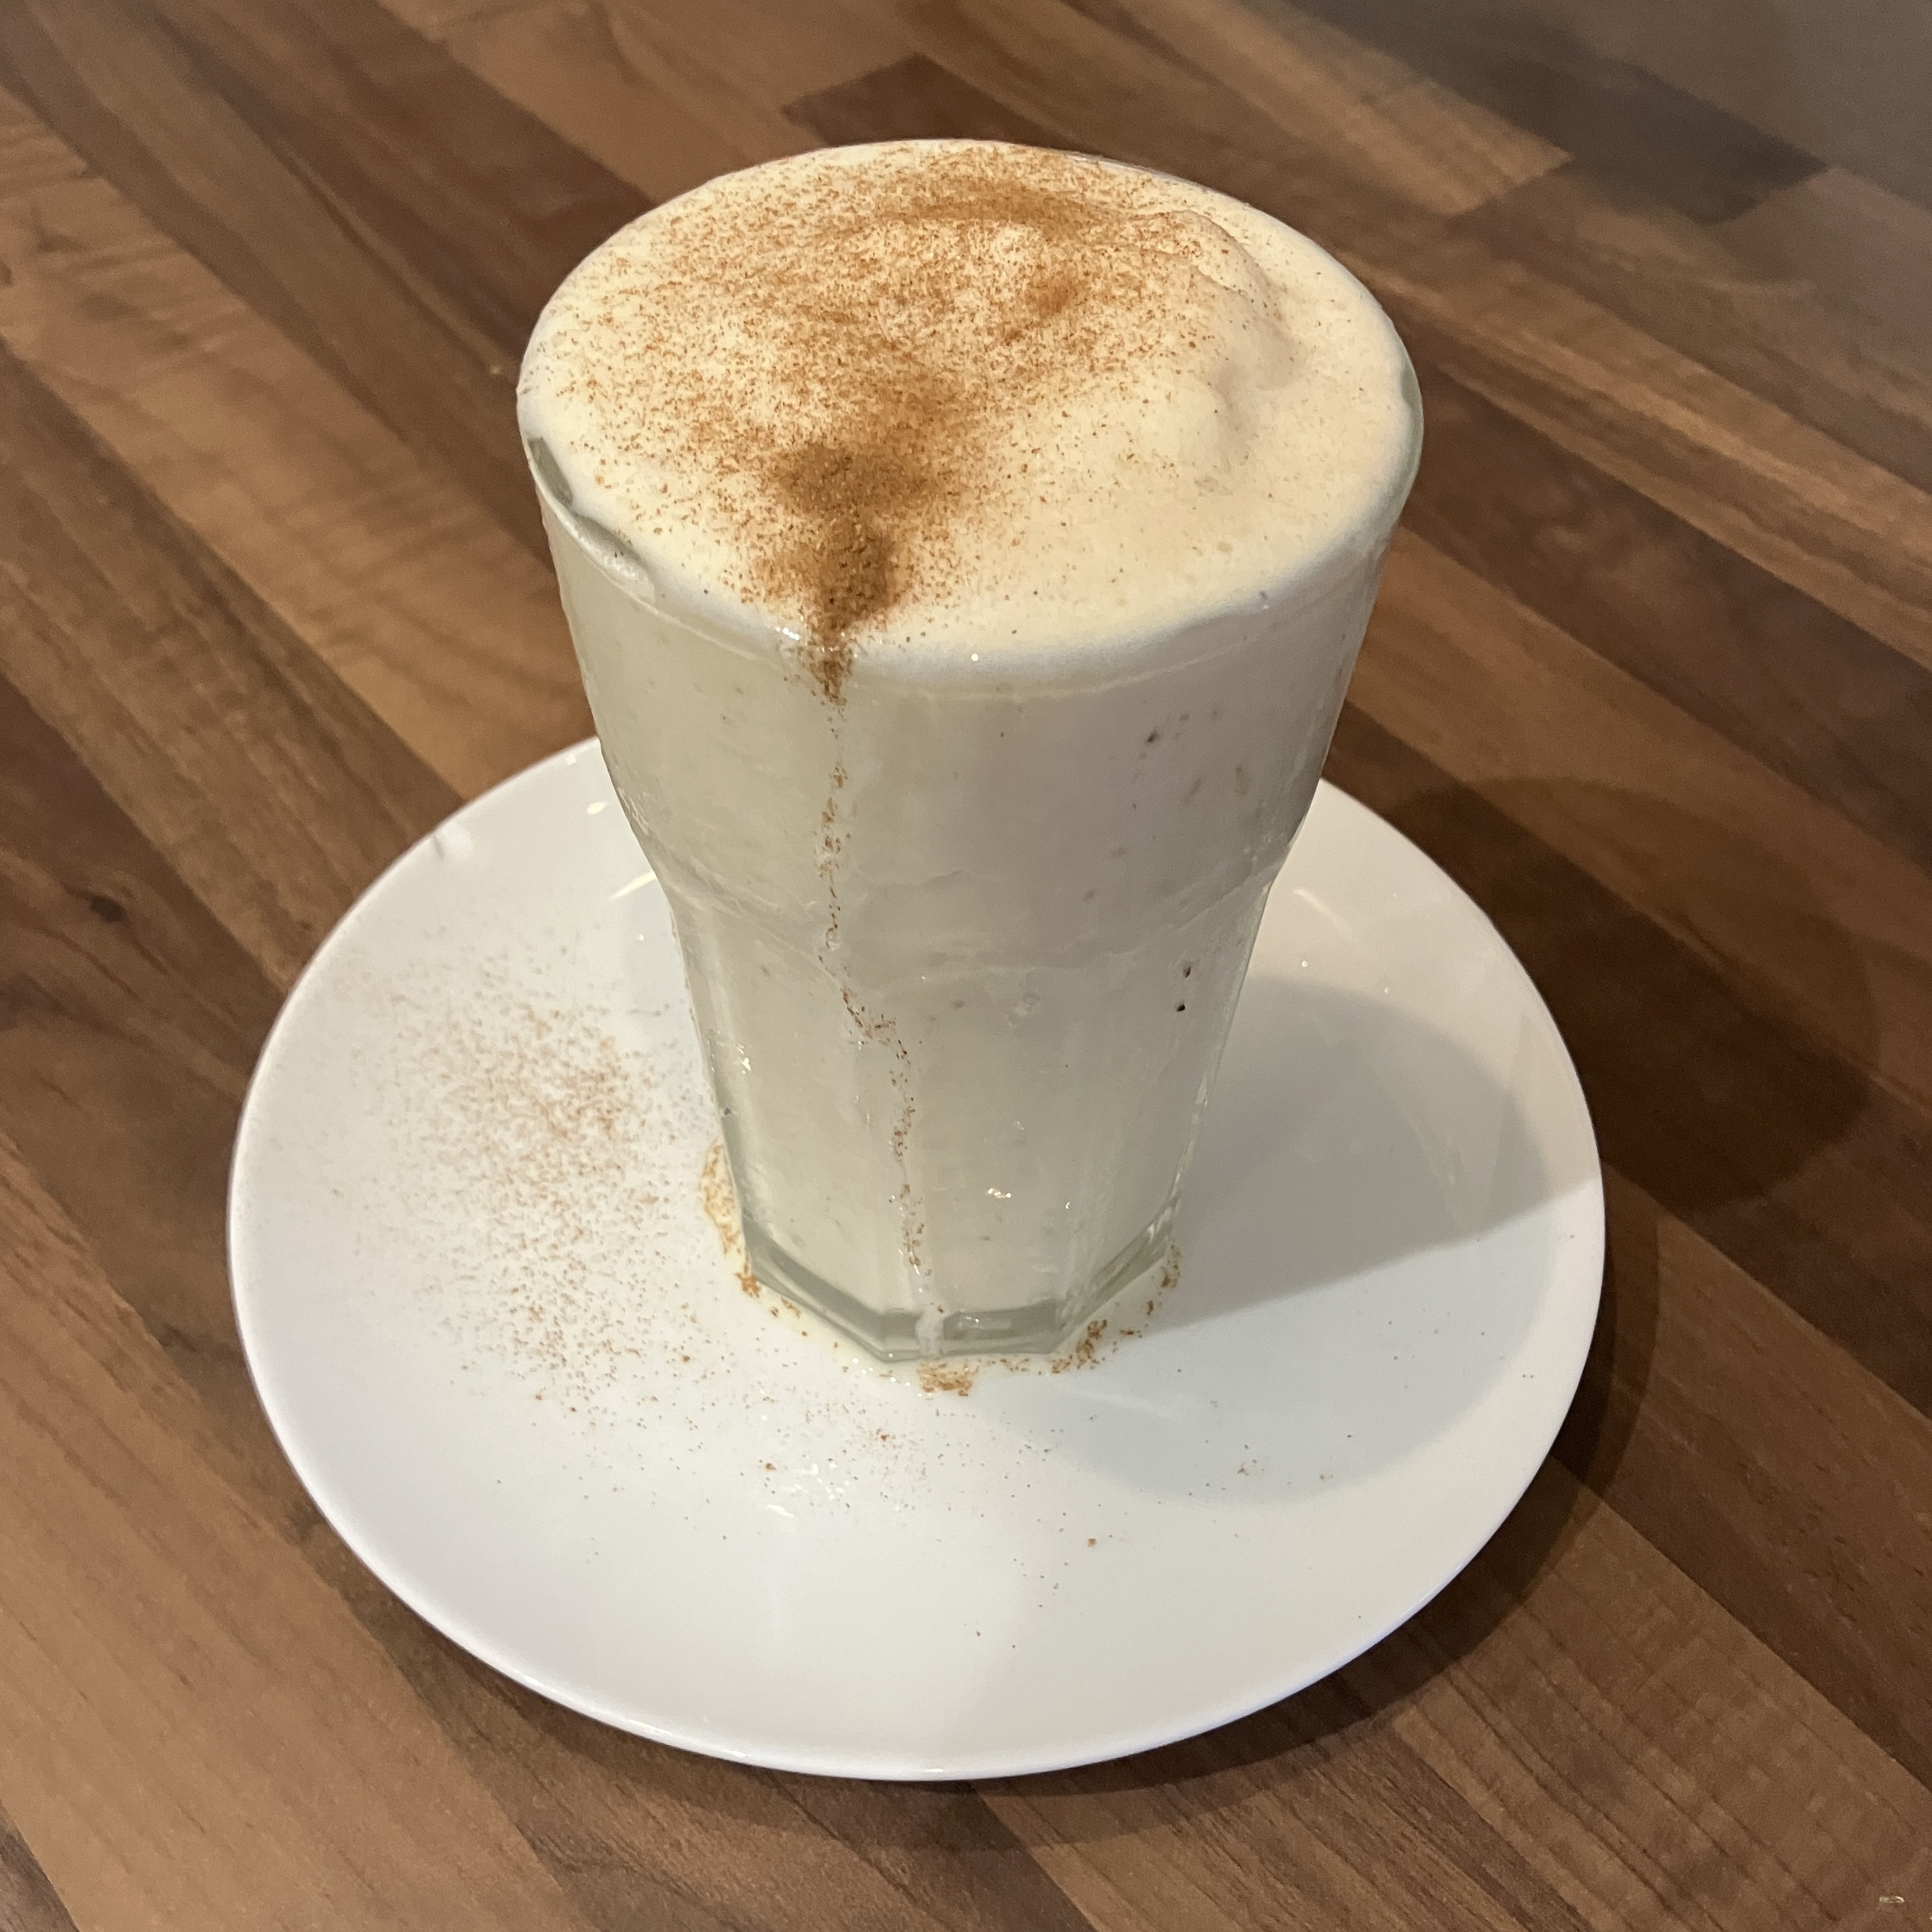
\includegraphics[width=\linewidth]{images/2025-10-12-banana-milkshake.jpg}}%
  
  		% Draw a clipping rectangle with rounded corners
  		\path[clip, rounded corners=0.5cm] (0,0) rectangle (\wd0,\ht0);
  
  		% Place the image inside the clipped area
  		\node[inner sep=0pt, outer sep=0pt, anchor=south west] at (0,0) {\usebox0};
	\end{tikzpicture}

  	\caption*{Jack's Banana milkshake, October 12, 2025.}
\end{figure}

